%%%%%%%%%%%%%%%%%%%%%%%%%%%%%%%%%%%%%%%%%%%%%%%%%%%%%%%%%%%%%%%%%%%%%%
% Template de Artigo
% XXIX ENMC – Encontro Nacional de Modelagem Computacional
% XVII ECTM – Encontro de Ciência e Tecnologia de Materiais
%%%%%%%%%%%%%%%%%%%%%%%%%%%%%%%%%%%%%%%%%%%%%%%%%%%%%%%%%%%%%%%%%%%%%%

\documentclass[12pt,fleqn]{article}

%%%%%%%%%%%%%%%%%%%%%%%%%%%%%%%%%%%%%%%%%%%%%%%%%%%%%%%%%%%%%%%%%%%%%%
% CONFIGURAÇÃO DE IDIOMA E CODIFICAÇÃO
%%%%%%%%%%%%%%%%%%%%%%%%%%%%%%%%%%%%%%%%%%%%%%%%%%%%%%%%%%%%%%%%%%%%%%

\usepackage[utf8]{inputenc}
\usepackage[T1]{fontenc}
\usepackage[brazil]{babel}

%%%%%%%%%%%%%%%%%%%%%%%%%%%%%%%%%%%%%%%%%%%%%%%%%%%%%%%%%%%%%%%%%%%%%%
% PACOTES DO TEMPLATE
%%%%%%%%%%%%%%%%%%%%%%%%%%%%%%%%%%%%%%%%%%%%%%%%%%%%%%%%%%%%%%%%%%%%%%

\usepackage{setup/config}
\usepackage{natbib}
\usepackage{graphicx}
\usepackage{color}
\usepackage{wallpaper}
\usepackage{hyperref}
\usepackage{titlesec}
\usepackage{float}
\usepackage{fancyhdr}
\usepackage{booktabs}
\usepackage{siunitx}
\setlength{\headheight}{20.68497pt}
\addtolength{\topmargin}{-8.68497pt}

%%%%%%%%%%%%%%%%%%%%%%%%%%%%%%%%%%%%%%%%%%%%%%%%%%%%%%%%%%%%%%%%%%%%%%
% DIRETÓRIO DAS FIGURAS
%%%%%%%%%%%%%%%%%%%%%%%%%%%%%%%%%%%%%%%%%%%%%%%%%%%%%%%%%%%%%%%%%%%%%%

\graphicspath{{figures/}}

%%%%%%%%%%%%%%%%%%%%%%%%%%%%%%%%%%%%%%%%%%%%%%%%%%%%%%%%%%%%%%%%%%%%%%
% AJUSTE DE ESPAÇAMENTO NA BIBLIOGRAFIA
%%%%%%%%%%%%%%%%%%%%%%%%%%%%%%%%%%%%%%%%%%%%%%%%%%%%%%%%%%%%%%%%%%%%%%

\let\OLDthebibliography\thebibliography
\renewcommand\thebibliography[1]{%
\OLDthebibliography{#1}
\setlength{\parskip}{0pt}
\setlength{\itemsep}{0pt plus 0.3ex}
}

%%%%%%%%%%%%%%%%%%%%%%%%%%%%%%%%%%%%%%%%%%%%%%%%%%%%%%%%%%%%%%%%%%%%%%
% TÍTULO DO ARTIGO
%%%%%%%%%%%%%%%%%%%%%%%%%%%%%%%%%%%%%%%%%%%%%%%%%%%%%%%%%%%%%%%%%%%%%%

\title{SISTEMA DE RECUPERAÇÃO AUTO ROTATIVO BIOINSPIRADO (SRAB) PARA NANOSSATÉLITE POCKETQUBE 1P: FUNDAMENTAÇÃO, MODELAGEM, VALIDAÇÃO EXPERIMENTAL PRELIMINAR E SIMULAÇÃO COMPUTACIONAL}

%%%%%%%%%%%%%%%%%%%%%%%%%%%%%%%%%%%%%%%%%%%%%%%%%%%%%%%%%%%%%%%%%%%%%%
% AUTORES E AFILIAÇÕES
%%%%%%%%%%%%%%%%%%%%%%%%%%%%%%%%%%%%%%%%%%%%%%%%%%%%%%%%%%%%%%%%%%%%%%

\author{Diego dos Santos Alves, et al.}



%%%%%%%%%%%%%%%%%%%%%%%%%%%%%%%%%%%%%%%%%%%%%%%%%%%%%%%%%%%%%%%%%%%%%%
% RODAPÉ ESPECIAL DA PRIMEIRA PÁGINA
%%%%%%%%%%%%%%%%%%%%%%%%%%%%%%%%%%%%%%%%%%%%%%%%%%%%%%%%%%%%%%%%%%%%%%

\fancypagestyle{firstpagestyle}
{
\renewcommand{\headrulewidth}{0pt}

\fancyfoot[C]{
\footnotesize
\parbox{15cm}{
\centering
\fontsize{7.5}{0}\selectfont\it
XXIX ENMC -- Encontro Nacional de Modelagem Computacional\\
XVII ECTM -- Encontro de Ciência e Tecnologia de Materiais\\
06 a 09 de outubro de 2026 - Bento Gonçalves - RS
}}
}

%%%%%%%%%%%%%%%%%%%%%%%%%%%%%%%%%%%%%%%%%%%%%%%%%%%%%%%%%%%%%%%%%%%%%%
% INÍCIO DO DOCUMENTO
%%%%%%%%%%%%%%%%%%%%%%%%%%%%%%%%%%%%%%%%%%%%%%%%%%%%%%%%%%%%%%%%%%%%%%

\begin{document}

\pretolerance=10000

%%%%%%%%%%%%%%%%%%%%%%%%%%%%%%%%%%%%%%%%%%%%%%%%%%%%%%%%%%%%%%%%%%%%%%
% LOGO DO EVENTO
%%%%%%%%%%%%%%%%%%%%%%%%%%%%%%%%%%%%%%%%%%%%%%%%%%%%%%%%%%%%%%%%%%%%%%

\begin{figure}
\centering

\includegraphics[width=6.25in]{logo.png}
\end{figure}

\vspace{-3cm}

%%%%%%%%%%%%%%%%%%%%%%%%%%%%%%%%%%%%%%%%%%%%%%%%%%%%%%%%%%%%%%%%%%%%%%
% TÍTULO
%%%%%%%%%%%%%%%%%%%%%%%%%%%%%%%%%%%%%%%%%%%%%%%%%%%%%%%%%%%%%%%%%%%%%%

\maketitle

\pagestyle{empty}
\thispagestyle{firstpagestyle}

%%%%%%%%%%%%%%%%%%%%%%%%%%%%%%%%%%%%%%%%%%%%%%%%%%%%%%%%%%%%%%%%%%%%%%
% RESUMO
%%%%%%%%%%%%%%%%%%%%%%%%%%%%%%%%%%%%%%%%%%%%%%%%%%%%%%%%%%%%%%%%%%%%%%

\begin{abstract}
A recuperação de nanossatélites PocketQube 1P depende tradicionalmente de paraquedas, que apresentam pontos únicos de falha como erros de dobradura, costura ou corrosão. Este trabalho propõe o Sistema de Recuperação Auto Rotativo Bioinspirado (SRAB), baseado no mecanismo de autorrotação passiva observado em sementes de samara (\textit{Acer rubrum}, \textit{Fraxinus}). O sistema utiliza arquitetura estrutural assimétrica que induz rotação cônica sem atuação ativa, gerando um Vórtice de Bordo de Ataque (LEV) que reduz a velocidade terminal. A validação emprega modelo dinâmico de quarta ordem (Newton-Euler reduzido) acoplado à Teoria do Elemento de Pá (BEM), implementado no simulador Samara PQ em Python, e ensaios experimentais de queda livre qualitativos com dois protótipos iterativos (Testes 1 e 2). A simulação computacional da configuração Asa3.DXF com 4 asas (Teste 3 -- Parte A) resultou em velocidade de impacto de 12,90~m/s, conicidade de equilíbrio de 17,22$^\circ$ e spin de 372~RPM. Análise de dispersão por Monte Carlo (200 iterações) indicou velocidade de impacto de 12,89~$\pm$~0,20~m/s (P95~=~13,19~m/s). A instrumentação embarcada (ESP32-C3, ICM-20602, BMP280, LoRa RFM95W) foi validada funcionalmente em 20~Hz.
\end{abstract}

\begin{keywords}
Recuperação passiva, samara, PocketQube, autorrotação, Monte Carlo
\end{keywords}

%%%%%%%%%%%%%%%%%%%%%%%%%%%%%%%%%%%%%%%%%%%%%%%%%%%%%%%%%%%%%%%%%%%%%%
% CABEÇALHO DAS DEMAIS PÁGINAS
%%%%%%%%%%%%%%%%%%%%%%%%%%%%%%%%%%%%%%%%%%%%%%%%%%%%%%%%%%%%%%%%%%%%%%

\fancyhead[L]{\footnotesize{\fontsize{7.5}{0}\selectfont\it
XXIX ENMC, XVII ECTM\\
06 a 09 de outubro de 2026}}

\renewcommand{\headrulewidth}{0pt}

\fancyfoot[C]{
\footnotesize
\parbox{15cm}{
\centering
\fontsize{7.5}{0}\selectfont\it
XXIX ENMC -- Encontro Nacional de Modelagem Computacional\\
XVII ECTM -- Encontro de Ciência e Tecnologia de Materiais\\
06 a 09 de outubro de 2026 - Bento Gonçalves - RS
}}

\rhead{}

\pagestyle{fancy}

%%%%%%%%%%%%%%%%%%%%%%%%%%%%%%%%%%%%%%%%%%%%%%%%%%%%%%%%%%%%%%%%%%%%%%
% SEÇÕES DO ARTIGO
%%%%%%%%%%%%%%%%%%%%%%%%%%%%%%%%%%%%%%%%%%%%%%%%%%%%%%%%%%%%%%%%%%%%%%

%%%%%%%%%%%%%%%%%%%%%%%%%%%%%%%%%%%%%%%%%%%%%%%%%%%%%%%%%%%%%%%%%%%%%%
% 1. INTRODUÇÃO
%%%%%%%%%%%%%%%%%%%%%%%%%%%%%%%%%%%%%%%%%%%%%%%%%%%%%%%%%%%%%%%%%%%%%%

\section{INTRODUÇÃO}

O regulamento da \textit{Latin American Space Challenge} (LASC) exige que os sistemas de recuperação de nanossatélites mantenham a descida controlada entre 20~m/s e 45~m/s \citep{lasc2026}. Embora comuns, os paraquedas apresentam pontos únicos de falha associados a costuras, dobraduras e mecanismos de acionamento. Como alternativa puramente passiva, este trabalho propõe o Sistema de Recuperação Auto Rotativo Bioinspirado (SRAB), inspirado na mecânica de voo de sementes de samara (\textit{Acer rubrum}, \textit{Fraxinus}). A assimetria estrutural dessas sementes induz uma rotação cônica estável, gerando Vórtices de Bordo de Ataque (LEV) que ampliam significativamente a sustentação sem o uso de atuadores \citep{lentink2009, mcconnell2023}.

Os objetivos específicos desta pesquisa são: (a) validar qualitativamente o modelo dinâmico de 4$^{\underline{a}}$ ordem do SRAB via ensaios de queda com protótipos iterativos (Testes 1 e 2); (b) projetar e validar a instrumentação embarcada para telemetria a 20~Hz (Teste 3 -- Parte B); (c) simular a configuração Asa3 (4 asas) em altitude operacional, incluindo análise de dispersão via Monte Carlo (Teste 3 -- Parte A); (d) conduzir análise de sensibilidade dos coeficientes aerodinâmicos no regime estacionário; e (e) comparar o desempenho do SRAB com o de um paraquedas equivalente.

O escopo delimita-se à demonstração de viabilidade física e à validação preliminar conceitual. O estudo não visa esgotar a caracterização quantitativa do regime terminal, mas estabelecer uma base teórica e instrumental robusta para futuras investigações e testes de lançamento em altitude operacional.

%%%%%%%%%%%%%%%%%%%%%%%%%%%%%%%%%%%%%%%%%%%%%%%%%%%%%%%%%%%%%%%%%%%%%%
% 2. FUNDAMENTAÇÃO TEÓRICA
%%%%%%%%%%%%%%%%%%%%%%%%%%%%%%%%%%%%%%%%%%%%%%%%%%%%%%%%%%%%%%%%%%%%%%

\section{FUNDAMENTAÇÃO TEÓRICA}

Esta seção fundamenta o projeto do SRAB, abordando o mecanismo de autorrotação passiva das sementes de samara, o Vórtice de Bordo de Ataque (LEV) e os modelos matemáticos de aerodinâmica e dinâmica do sistema.

\subsection{Autorrotação passiva em sementes de samara}

Sementes do tipo \textit{samara} são estruturas aladas cuja assimetria estrutural induz rotação estável em torno do eixo vertical ao caírem \citep{limacher2015}. Essa autorrotação passiva gera sustentação, reduz a velocidade terminal e favorece a dispersão horizontal, descrita pela relação \citep{limacher2015}:
\begin{equation}
x_h = h \cdot \frac{v_w}{v_s}
\end{equation}
A cinemática de equilíbrio é caracterizada por dois parâmetros adimensionais: o número de Reynolds ($Re$) e a razão de velocidade de ponta ($\lambda$) \citep{limacher2015}:
\begin{equation}
\lambda = \frac{\Omega \, R_d}{v_0}
\qquad
Re = \frac{c\,\sqrt{v_0^2 + (\Omega R_d)^2}}{\nu}
\end{equation}
A estabilidade longitudinal é mantida com um ângulo de conicidade $\beta$ entre 13$^{\circ}$ e 35$^{\circ}$, e o centro de massa posicionado entre 27\% e 35\% da corda a partir do bordo de ataque \citep{limacher2015}.

\subsection{Vórtice de bordo de ataque (LEV)}

O mecanismo aerodinâmico central da autorrotação é o Vórtice de Bordo de Ataque (\textit{Leading-Edge Vortex}, LEV). Ao contrário das asas convencionais, que sofrem \textit{estol} em altos ângulos de ataque, a rotação mantém o escoamento no extradorso aderido \citep{lentink2009, rezgui2020}.

Lentink et al. \citeyear{lentink2009} mostraram que o escoamento radial (\textit{spanwise flow}) drena a vorticidade para a ponta da asa, estabilizando a estrutura do LEV. Isso resulta em coeficientes de sustentação locais excepcionais na região basal (entre 2 e 5), superando amplamente o limite de \textit{estol} \citep{lentink2009, mcconnell2023}.

\subsection{Modelo de sustentação sectional do LEV}

Para incorporar o efeito do LEV, Rezgui et al. \citeyear{rezgui2020} adaptaram o método de Polhamus. Assumindo a sustentação total como a soma das componentes potencial e vortex, a expressão sectional torna-se:
\begin{equation}
C_l(\alpha) = K_p \sin(\alpha) \cos^2(\alpha) + K_v \cos(\alpha) \sin^2(\alpha)
\end{equation}
A polar resultante apresenta sustentação superior à do escoamento potencial, atingindo máximos próximos a $\alpha \approx 45^{\circ}$. Uma correção bidimensional via teoria de Prandtl pode ser aplicada para converter a polar 3-D em coeficiente seccional local \citep{rezgui2020}.

\subsection{Modelo de Elemento de Pá (BEM) e dinâmica do SRAB}

No SRAB, as forças aerodinâmicas são calculadas pela Teoria do Elemento de Pá (BEM). As forças elementares de sustentação ($\delta L$) e arrasto ($\delta D$) seguem a polar de Polhamus:
\begin{equation}
\delta L = \frac{1}{2} \rho \, U^2 \, c \, \delta r \, C_l(\alpha)
\qquad
\delta D = \frac{1}{2} \rho \, U^2 \, c \, \delta r \, C_d
\end{equation}
McConnell e Das \citeyear{mcconnell2023} descrevem a dinâmica dessas sementes por um modelo de 4$^{\underline{a}}$ ordem, cujo vetor de estado engloba o ângulo de conicidade ($\theta$), as taxas de arfagem ($\dot\theta$) e guinada ($\dot\phi$), e a velocidade de descida ($v_0$):
\begin{equation}
\ddot\theta = -\frac{M_{y3}}{I_{y3y3}} - \dot\phi^2 \sin\theta \cos\theta
\qquad
\ddot\phi = \frac{M_{z3}}{I_{y3y3} \cos\theta} + 2\,\dot\phi\,\dot\theta \tan\theta
\end{equation}
\begin{equation}
\dot{v}_0 = -g + \frac{F_{z3} \cos\theta}{m}
\end{equation}
As equações de Newton-Euler capturam o momento de restauração cônica e o acoplamento giroscópico típicos da autorrotação. A baixa inércia do SRAB permite rápido reajuste frente a rajadas, mantendo a estabilidade dinâmica do sistema \citep{limacher2015, mcconnell2023}.  % §1 Introdução + §2 Fundamentação Teórica
%%%%%%%%%%%%%%%%%%%%%%%%%%%%%%%%%%%%%%%%%%%%%%%%%%%%%%%%%%%%%%%%%%%%%%
% 3. MATERIAIS E MÉTODOS
%%%%%%%%%%%%%%%%%%%%%%%%%%%%%%%%%%%%%%%%%%%%%%%%%%%%%%%%%%%%%%%%%%%%%%

\section{MATERIAIS E MÉTODOS}

\subsection{Simulação computacional (Pipeline Samara PQ)}

O simulador Samara PQ, desenvolvido em Python, integra numericamente o modelo dinâmico da Seção 2.4 para reproduzir a trajetória de queda até o impacto. O processo inicia-se com a importação de contornos geométricos de arquivos DXF (biblioteca \texttt{ezdxf}), extraindo-se automaticamente o perfil de corda, a área total e o raio efetivo da asa.

A resolução das equações diferenciais utiliza o método Runge--Kutta de 5$^{\underline{a}}$ ordem (\texttt{solve\_ivp}, RK45, da biblioteca SciPy), selecionado por oferecer controle adaptativo de passo e estabilidade numérica, características essenciais para lidar com a dinâmica multi-escala do SRAB. Ao final, o ambiente exporta os resultados em relatórios numéricos (JSON e TXT) e gera gráficos temporais do comportamento das variáveis de estado, como altitude, velocidade, ângulo de conicidade e rotação.

\subsection{Ensaios experimentais qualitativos (Testes 1 e 2)}

Protótipos físicos montados sob a plataforma Alba Orbital 1P foram submetidos a quedas livres a partir de drone em altitude máxima de aproximadamente 20~m. O primeiro protótipo, Teste 1, utilizou quatro asas com área total de 109,22~cm$^2$ (asa1.dxf), apresentando sustentação detectável embora com desalinhamento estrutural evidente durante a rotação. Com base nas observações do Teste 1, a geometria foi otimizada para o Teste 2, que empregou a Asa2.DXF com 122,28~cm$^2$, um aumento de 12\% na área, e resultou em rotação cônica visualmente mais estável.

A Tabela~\ref{tab:testes12} apresenta os parâmetros de simulação para os Testes 1 e 2.

\begin{table}[h]
\caption{Parâmetros de simulação computacional para os Testes 1 e 2. Condições: queda de 20~m, massa 200~g, $\beta=8^\circ$, $C_{D0}=1,0$, $f_{factor}=0,3$, $\rho=1,225$~kg/m$^3$.}
\centering
\begin{tabular*}{\textwidth}{@{\extracolsep{\fill}}lccc}
\hline
Parâmetro & Teste 1 (Asa1, 4 asas) & Teste 2 (Asa2, 4 asas) & Variação \\
\hline
Área Total das Asas [cm$^2$] & 109,22 & 122,28 & +12\% \\
Velocidade de Impacto [m/s] & 7,68 & 8,04 & +4,7\% \\
Energia Cinética no Impacto [J] & 5,90 & 6,47 & +9,7\% \\
Tempo de Voo [s] & 2,79 & 2,70 & $-$3,2\% \\
Conicidade $\theta$ no Impacto [$^\circ$] & 13,46 & 24,44 & +81,6\% \\
Taxa de Rotação no Impacto [RPM] & 306,77 & 306,89 & +0,04\% \\
Número de Reynolds médio & 9\,875 & 13\,876 & +40,5\% \\
\hline
\end{tabular*}
{\footnotesize\centering Fonte: Autores (2026)\par}
\label{tab:testes12}
\end{table}

\subsection{Instrumentação embarcada (Teste 3 -- Parte B)}

Projetou-se uma suíte de telemetria com massa total de 15~g, composta por microcontrolador ESP32-C3, IMU ICM-20602 e barômetro BMP280 (ambos com amostragem a 20~Hz), além de transceptor LoRa RFM95W e data logger em memória flash (LittleFS). Um módulo GPS u-blox NEO-8M está previsto para integração futura, com a massa restante (3,5~g) alocada para bateria e suportes.

O firmware realiza leitura simultânea via I2C, cálculo da taxa de descida por derivada numérica, detecção automática de apogeu, filtragem de dados e armazenamento em formato CSV a 20~Hz. A integridade do sistema e a detecção de apogeu foram plenamente validadas em ensaios de bancada sem perda de amostras.

\subsection{Teste 3 -- Protocolo e estrutura}

O Teste 3 consiste na campanha de validação da configuração Asa3.DXF (4 asas), dividida em duas frentes complementares. A Parte A (cujos resultados constam na Seção 4.4) utiliza o simulador Samara PQ para caracterizar o regime estacionário a 1000~m de altitude, incluindo análise de robustez por Monte Carlo. 

A Parte B, que permanece como trabalho futuro, compreende o ensaio de campo com lançamento em altitude operacional e coleta de dados via telemetria (Seção 3.3). Para a validação, os critérios de aceitação estipulam erros máximos em relação às simulações da Parte A de $\pm5\%$ para a velocidade de impacto e $\pm3\%$ para o tempo de voo.  % §3 Materiais e Métodos
%%%%%%%%%%%%%%%%%%%%%%%%%%%%%%%%%%%%%%%%%%%%%%%%%%%%%%%%%%%%%%%%%%%%%%
% 4. RESULTADOS E DISCUSSÃO
%%%%%%%%%%%%%%%%%%%%%%%%%%%%%%%%%%%%%%%%%%%%%%%%%%%%%%%%%%%%%%%%%%%%%%

\section{RESULTADOS E DISCUSSÃO}

A Tabela~\ref{tab:resumo} resume os parâmetros de simulação para todos os testes.

\begin{table}[htbp]
\caption{Resumo dos parâmetros de simulação.}
\centering
\begin{tabular*}{\textwidth}{@{\extracolsep{\fill}}lcccc}
\hline
Parâmetro & Teste 1 & Teste 2 & Teste 3 & MC \\
\hline
DXF & asa1.dxf & Asa2.DXF & Asa3.DXF & Asa3.DXF \\
$n_{wings}$ & 4 & 4 & 4 & 4 \\
Massa [g] & 200 & 200 & 200 & 200 $\pm$ 10 \\
$\beta$ [$^\circ$] & 8 & 8 & 3 & 3 $\pm$ 0,5 \\
$C_{D0}$ & 1,0 & 1,0 & 1,0 & 1,0 $\pm$ 0,10 \\
$f_{factor}$ & 0,3 & 0,3 & 0,3 & 0,3 $\pm$ 0,03 \\
$\rho$ [kg/m$^3$] & 1,225 & 1,225 & 1,225 & 1,225 \\
Altitude [m] & 20 & 20 & 1000 & 1000 \\
Iterações & 1 & 1 & 1 & 200 \\
\hline
\end{tabular*}
{\footnotesize\centering Fonte: Autores (2026)\par}
\label{tab:resumo}
\end{table}

\subsection{Validação qualitativa (Testes 1 e 2)}

As Figuras~\ref{fig:test1_lrr} a~\ref{fig:test2_lrr} e a Tabela~\ref{tab:testes12} detalham os \textit{dashboards} LRR (\textit{Launch Readiness Review}) e os parâmetros simulados dos Testes 1 e 2. A comparação revela a não linearidade entre área aerodinâmica e torque restaurador: um acréscimo de apenas 12\% na área ampliou a conicidade de impacto em 81,6\% (de 13,46$^\circ$ para 24,44$^\circ$). Isso corrobora o modelo BEM, no qual o momento $M_{y3}$ escala com o quadrado da corda local.

A taxa de rotação inalterada ($\approx 306,8$~RPM) indica que a velocidade angular de equilíbrio é governada majoritariamente pelo ângulo de passo $\beta$ e pela distribuição de massa, sendo insensível à variação da área total. Por fim, o aumento de 40,5\% no número de Reynolds médio reflete a maior velocidade do Teste 2 (8,04~m/s ante 7,68~m/s), aproximando o escoamento do regime transicional turbulento, o que favorece a estabilidade do LEV \citep{rezgui2020}.

\begin{figure}[htbp]
\centering

\includegraphics[width=0.85\textwidth]{fig_test1_lrr.png}
\caption{LRR do Teste 1 (Asa1, 4 asas, 200~g).}
{\footnotesize\centering Fonte: Autores (2026)\par}
\label{fig:test1_lrr}
\end{figure}

% \begin{figure}[htbp]
% \centering
% 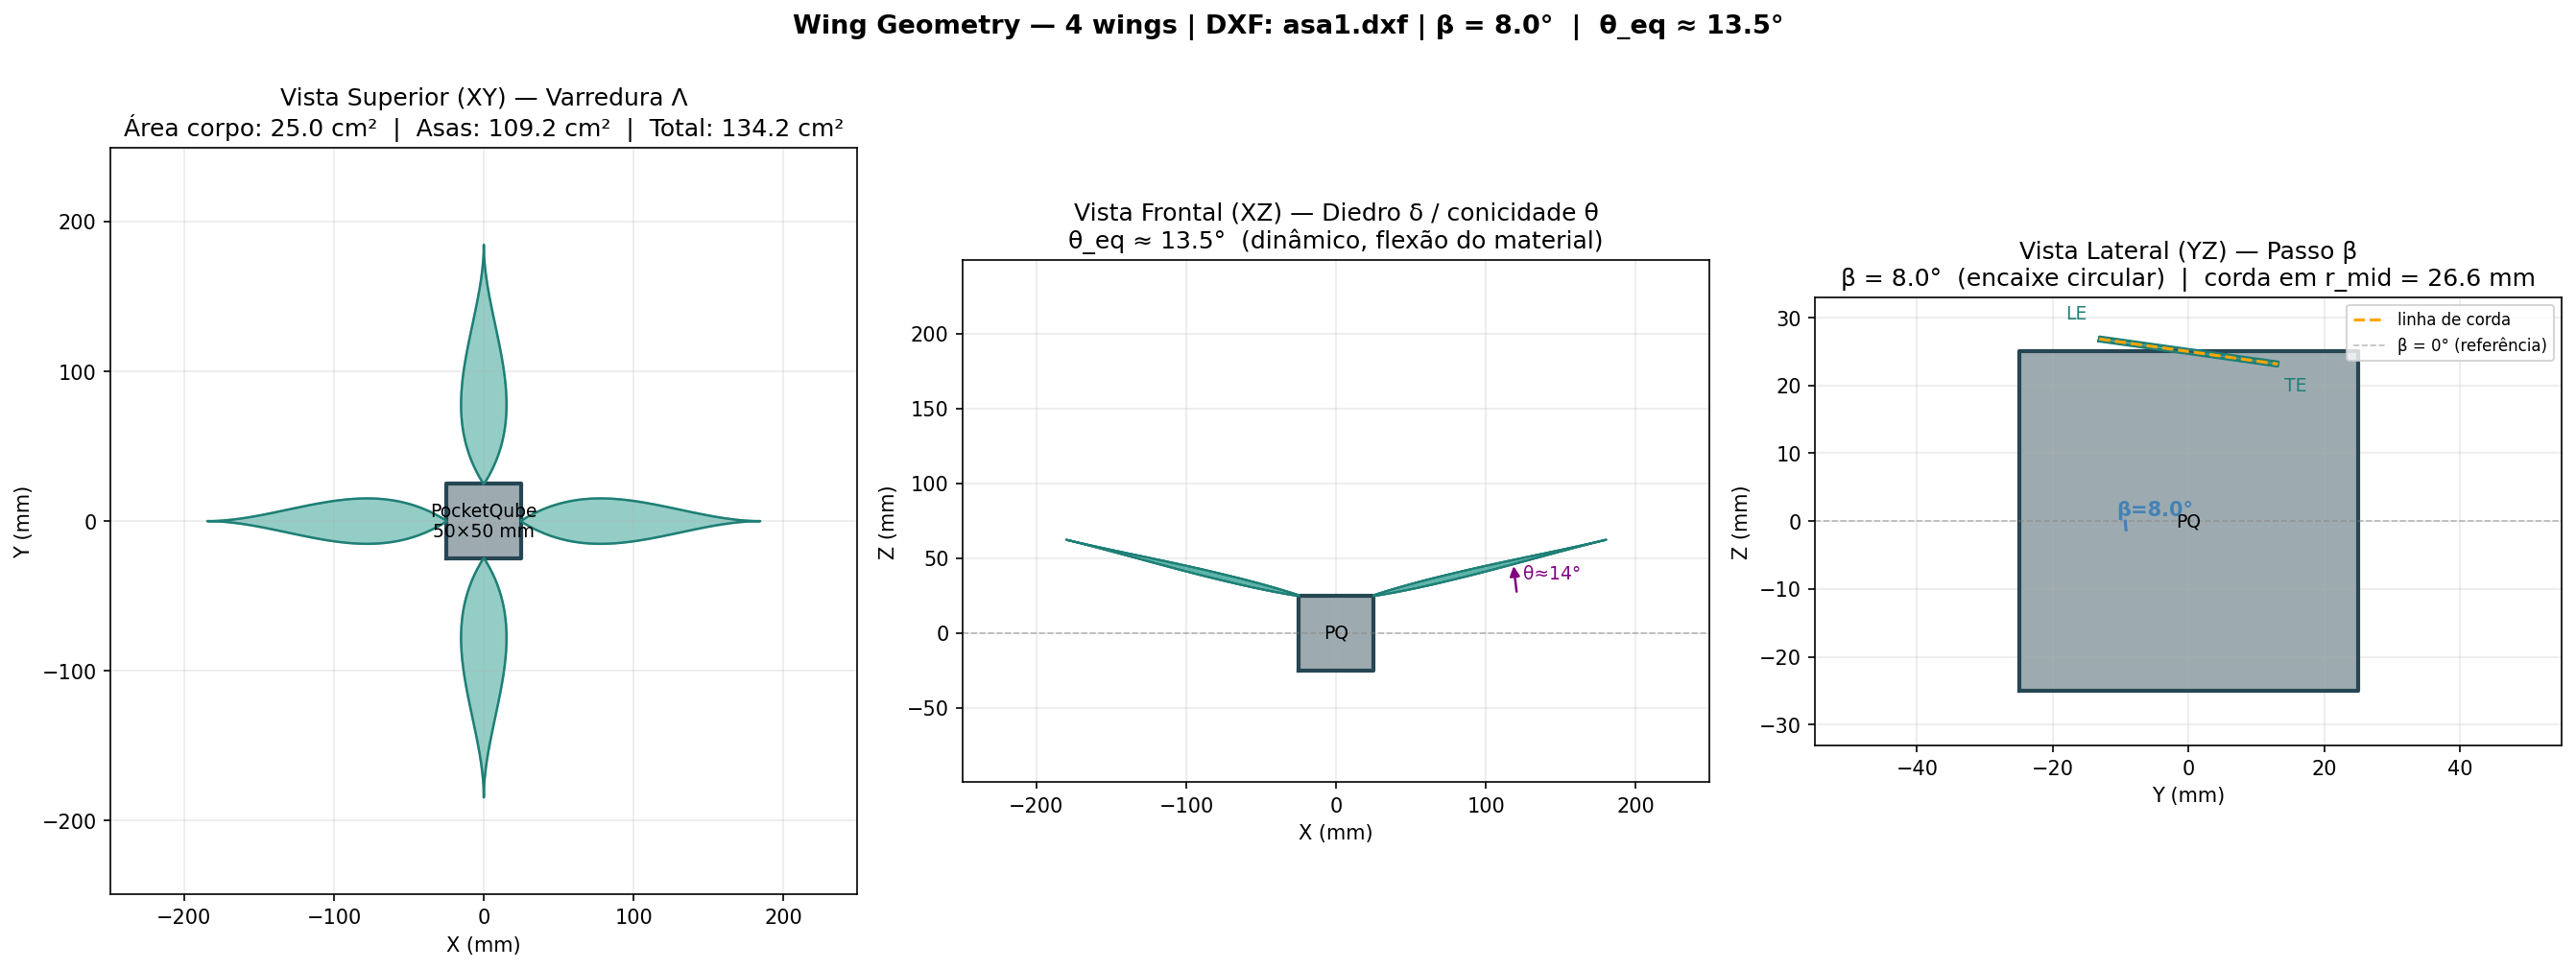
\includegraphics[width=0.85\textwidth]{fig_test1_geom.png}
% \caption{Vistas geométricas do Teste 1 (Asa1).}
% {\footnotesize\centering Fonte: Autores (2026)\par}
% \label{fig:test1_geom}
% \end{figure}

\begin{figure}[htbp]
\centering

\includegraphics[width=0.85\textwidth]{fig_test2_lrr.png}
\caption{LRR do Teste 2 (Asa2, 4 asas, 200~g).}
{\footnotesize\centering Fonte: Autores (2026)\par}
\label{fig:test2_lrr}
\end{figure}

% \begin{figure}[htbp]
% \centering
% 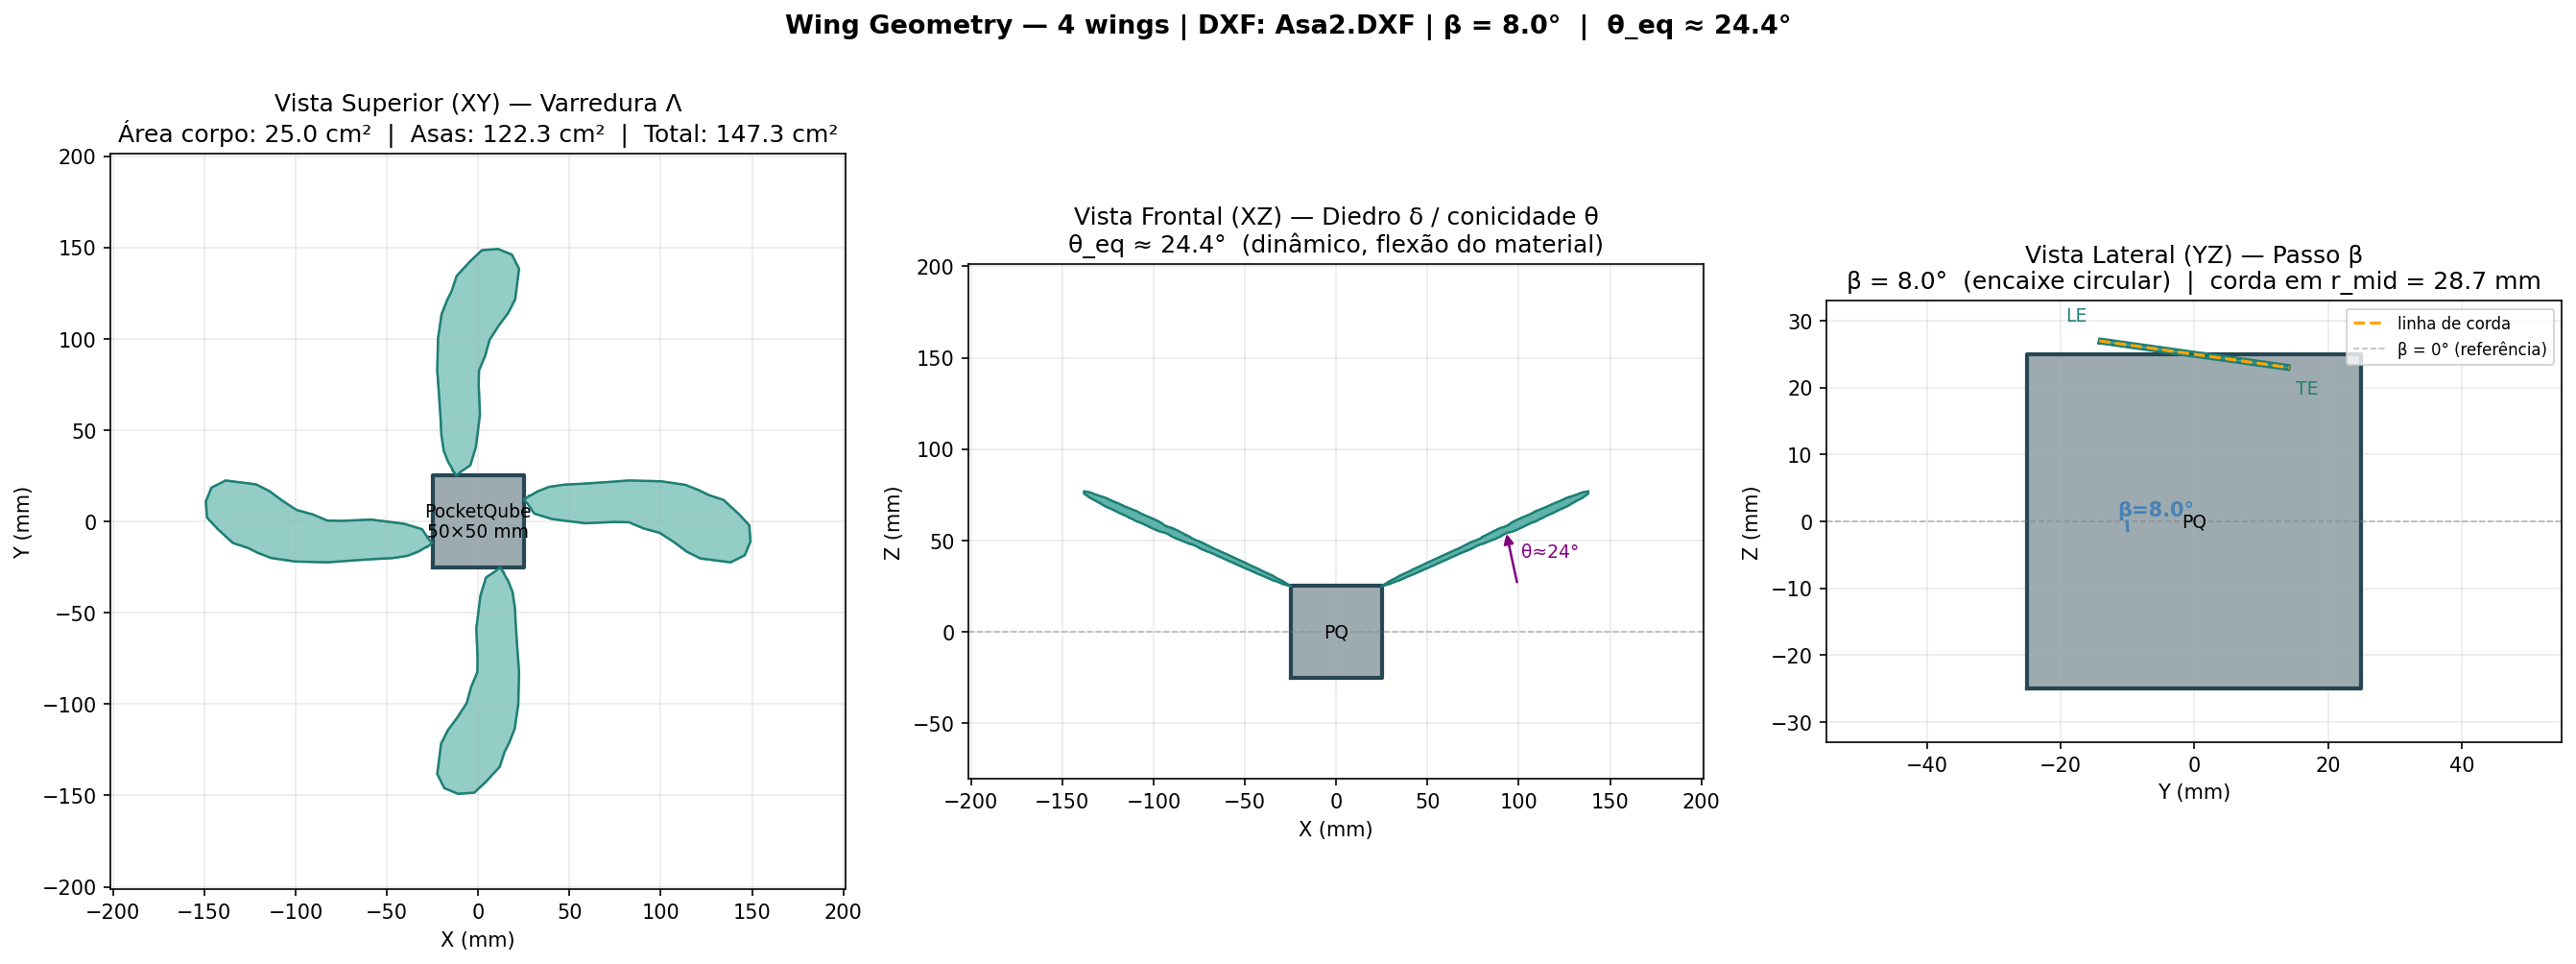
\includegraphics[width=0.85\textwidth]{fig_test2_geom.png}
% \caption{Vistas geométricas do Teste 2 (Asa2).}
% {\footnotesize\centering Fonte: Autores (2026)\par}
% \label{fig:test2_geom}
% \end{figure}

\subsection{Simulação em altitude operacional (Teste 3)}

A Tabela~\ref{tab:test3} e as Figuras~\ref{fig:test3_lrr} e~\ref{fig:test3_geom} detalham os resultados e vistas da configuração Asa3.DXF (4 asas) simulada a 1000~m. O sistema atinge velocidade de impacto de 12,90~m/s, conicidade de equilíbrio de 17,22$^\circ$ e taxa de rotação de 372~RPM.

\begin{table}[htbp]
\caption{Resultados da simulação computacional para o Teste 3 (Asa3, 4 asas).}
\centering
\begin{tabular*}{\textwidth}{@{\extracolsep{\fill}}lc}
\hline
Parâmetro & Valor \\
\hline
Geometria & Asa3.DXF, 4 asas \\
Massa total [g] & 200 \\
Velocidade de impacto [m/s] & 12,90 \\
 Tempo de descida [s] & 78,03 \\
Conicidade $\theta$ de equilíbrio [$^\circ$] & 17,22 \\
Taxa de rotação [RPM] & 371,98 \\
Energia cinética final [J] & 16,65 \\
Energia potencial inicial [J] & 1962,00 \\
Energia dissipada [J] (\%) & 1945,35 (99,15\%) \\
\hline
\end{tabular*}
{\footnotesize\centering Fonte: Autores (2026)\par}
\label{tab:test3}
\end{table}

A análise dinâmica destaca três aspectos: (1) a alta dissipação energética (99,15\%), restando apenas 16,65~J de energia cinética no impacto; (2) a redução da conicidade ante o Teste 2 (de 24,44$^\circ$ para 17,22$^\circ$), explicada pela diminuição do ângulo de passo $\beta$ (de 8$^\circ$ para 3$^\circ$); e (3) o tempo de voo de 78,03~s (taxa média de 12,82~m/s), atestando a rápida convergência à velocidade terminal.

Embora a velocidade final (12,90~m/s) situe-se abaixo da janela regulatória LASC (20--45~m/s), o conceito autorrotativo permanece válido, demandando apenas ajustes geométricos para o pleno enquadramento aos requisitos operacionais.

\begin{figure}[htbp]
\centering
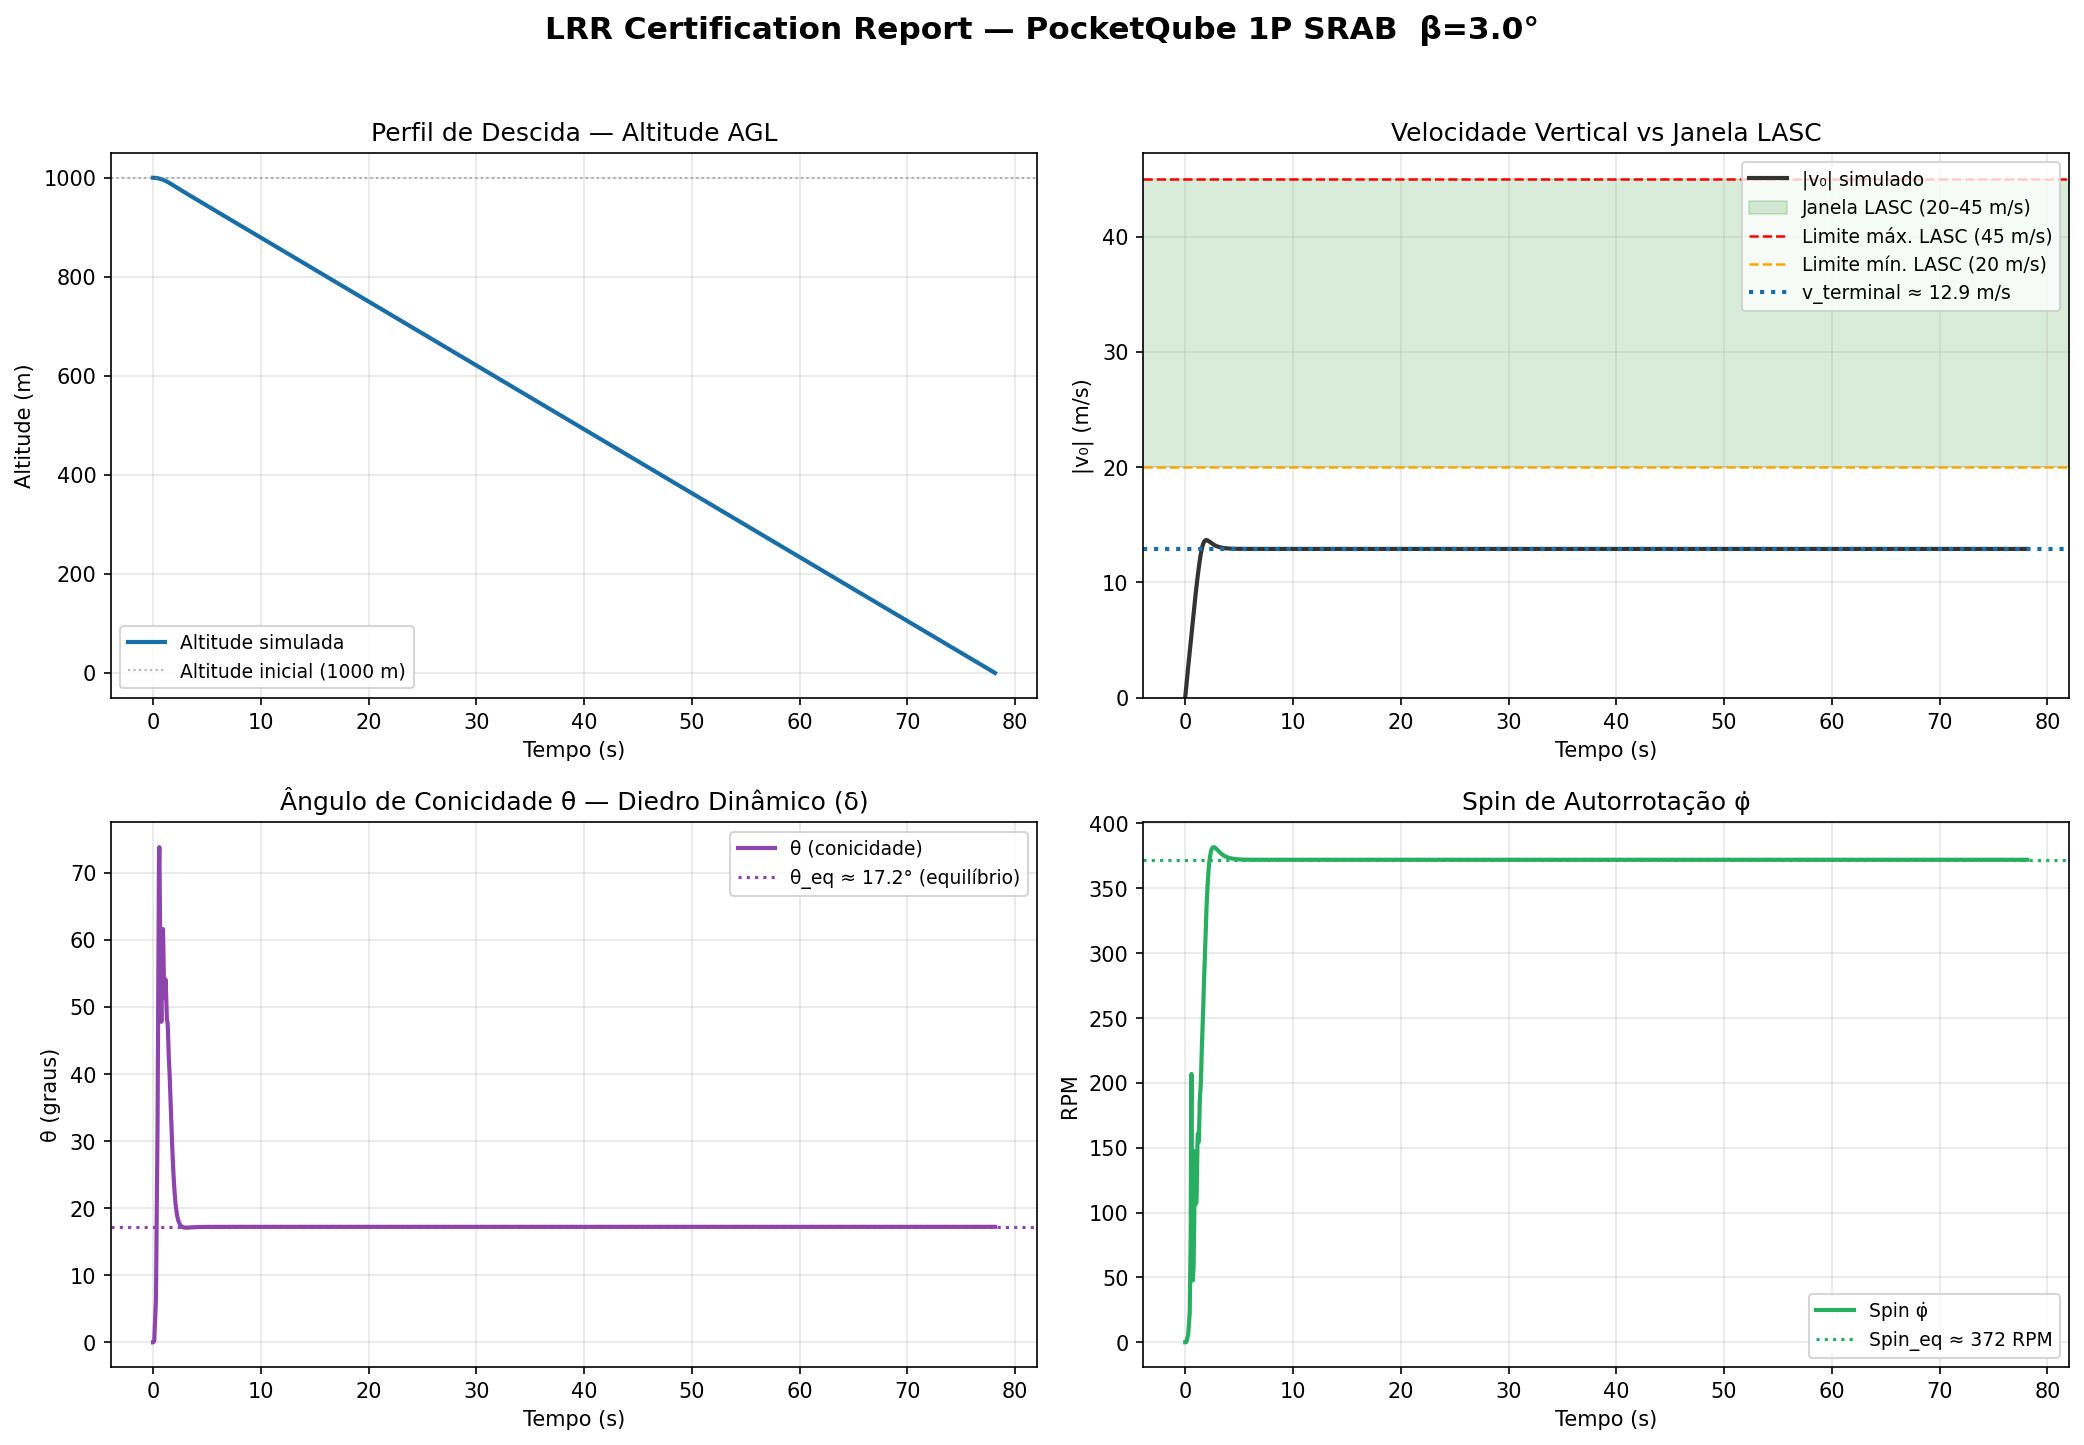
\includegraphics[width=0.85\textwidth]{fig_test3_lrr.png}
\caption{LRR do Teste 3 (Asa3, 4 asas, 200~g). Velocidade de impacto de 12,90~m/s com conicidade de 17,22$^\circ$.}
{\footnotesize\centering Fonte: Autores (2026)\par}
\label{fig:test3_lrr}
\end{figure}

\begin{figure}[htbp]
\centering
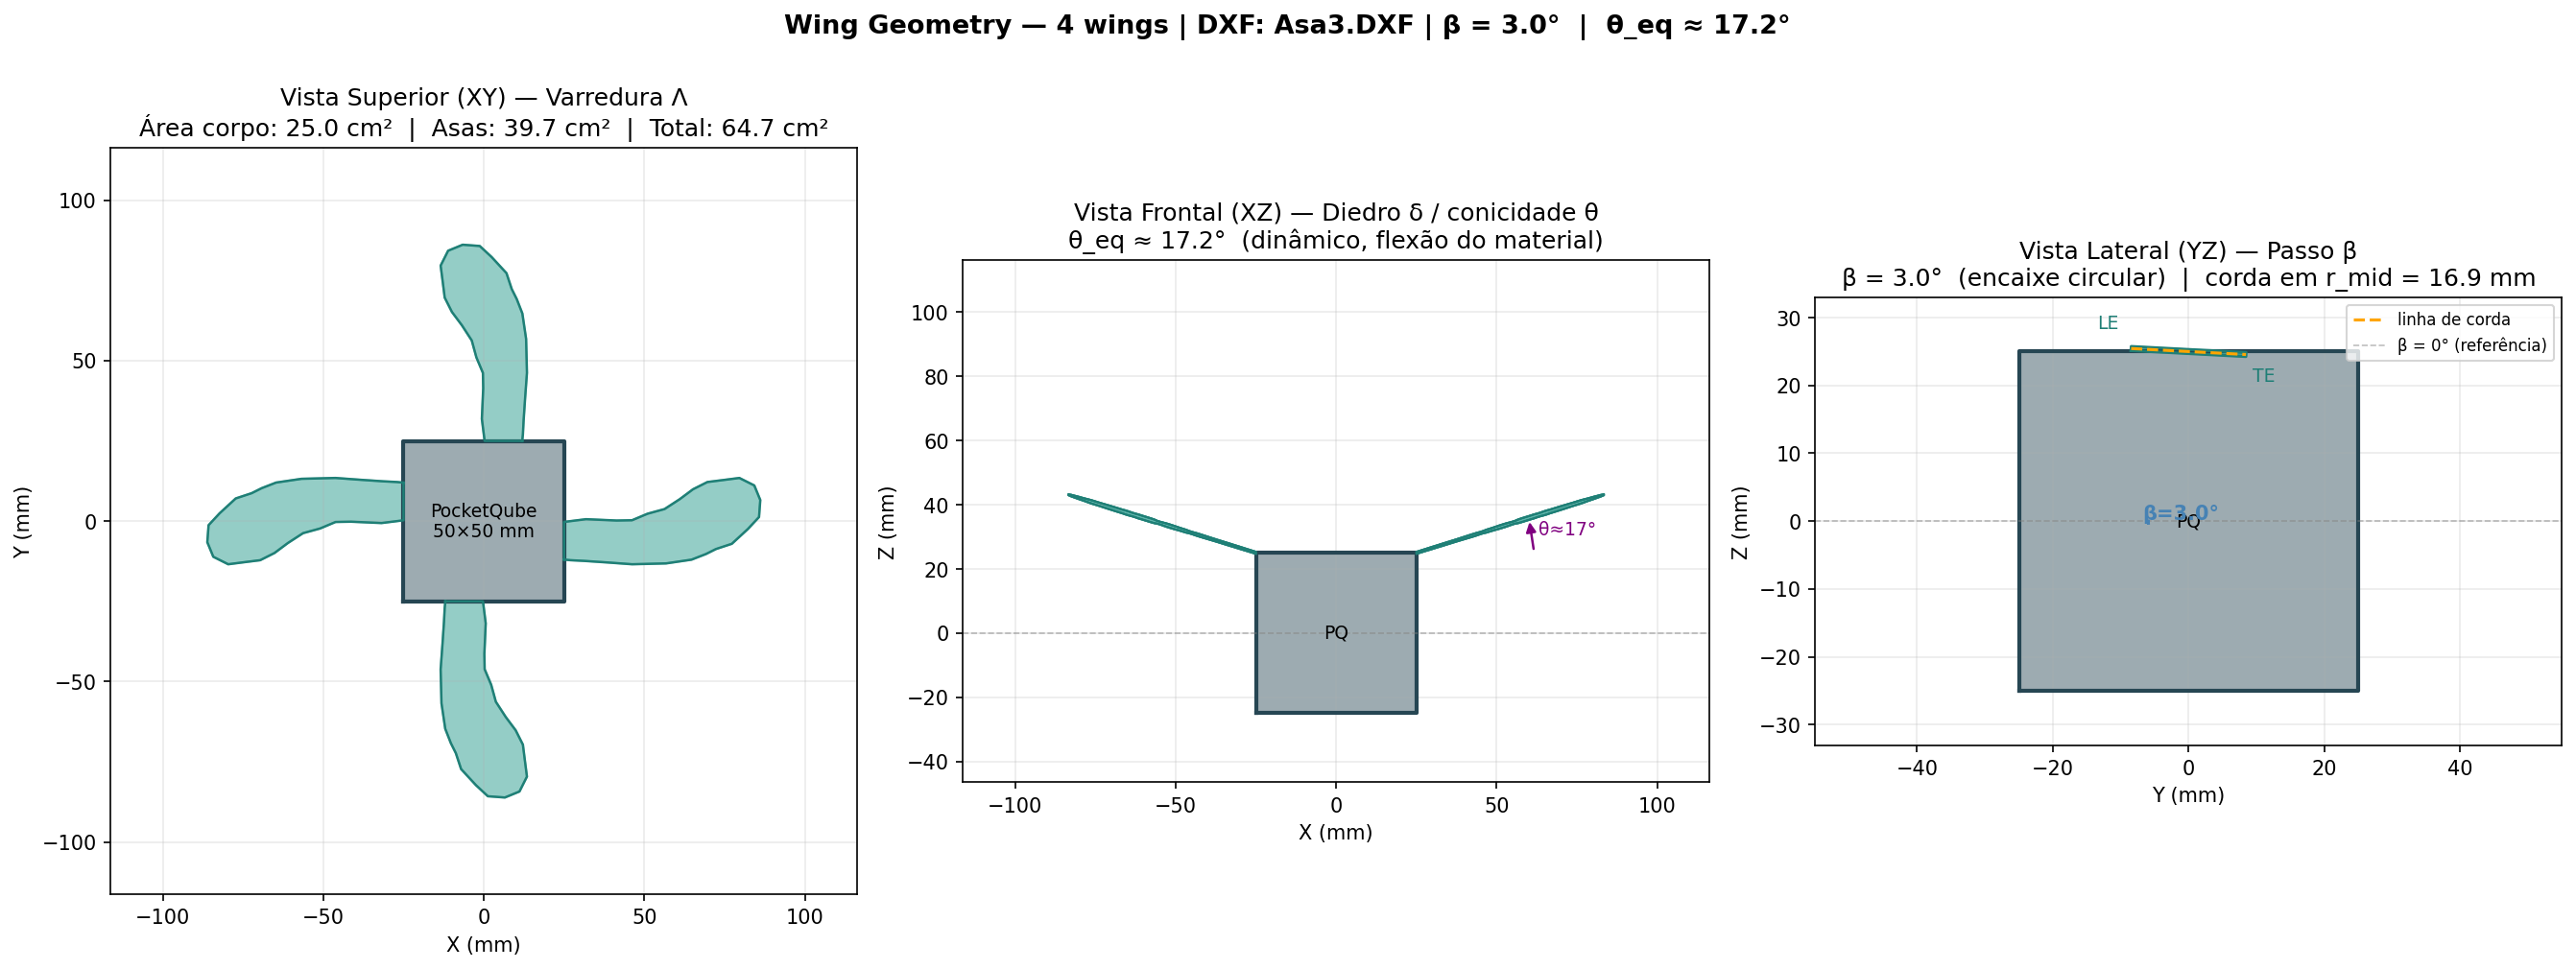
\includegraphics[width=0.85\textwidth]{fig_test3_geom.png}
\caption{Vistas geométricas do Teste 3 (Asa3, 4 asas).}
{\footnotesize\centering Fonte: Autores (2026)\par}
\label{fig:test3_geom}
\end{figure}

\subsection{Análise de sensibilidade do parâmetro $C_{D0}$}

A Tabela~\ref{tab:cd0} detalha a análise de sensibilidade variando $C_{D0}$ em $\pm10\%$ e $\pm20\%$ ante o valor calibrado ($C_{D0}=1,0$), mantendo fixos os demais parâmetros (Asa3.DXF, 4 asas, 200~g, $\beta=3^\circ$, altitude de 1000~m, $\rho=1,225$~kg/m$^3$, $f_{factor}=0,3$).

\begin{table}[htbp]
\caption{Análise de sensibilidade de $C_{D0}$ para a configuração Asa3 com 4 asas.}
\centering
\begin{tabular*}{\textwidth}{@{\extracolsep{\fill}}lccc}
\hline
$C_{D0}$ & Variação & Velocidade de Impacto [m/s] & Energia Cinética [J] \\
\hline
0,8 & $-$20\% & 12,90 & 16,65 \\
0,9 & $-$10\% & 12,90 & 16,65 \\
1,0 & nominal & 12,90 & 16,65 \\
1,1 & +10\% & 12,90 & 16,65 \\
1,2 & +20\% & 12,90 & 16,65 \\
\hline
\end{tabular*}
{\footnotesize\centering Fonte: Autores (2026)\par}
\label{tab:cd0}
\end{table}

A velocidade de impacto manteve-se inalterada na faixa testada, evidenciando que a sustentação aerodinâmica — e não o arrasto basal — é o mecanismo dominante na autorrotação. Esse comportamento corrobora a física do LEV: ao se estabelecer, a sustentação do vórtice sobrepuja fortemente o arrasto de forma, tornando o sistema robusto a variações de rugosidade superficial ou do perfil. Assim, embora o $C_{D0}$ seja relevante na aceleração inicial, ele perde influência assim que o regime cônico-estacionário é atingido.

\subsection{Análise de robustez Monte Carlo (Teste 3)}

Para quantificar a dispersão esperada, conduziu-se análise Monte Carlo com 200 iterações, variando simultaneamente a massa total (200~$\pm$~10~g), o ângulo de passo $\beta$ (3,0$^\circ$~$\pm$~0,5$^\circ$), $C_{D0}$ (1,0~$\pm$~0,10) e $f_{factor}$ (0,3~$\pm$~0,03). Os intervalos foram definidos com base nas tolerâncias de fabricação estimadas para impressão PETG a 0,6~mm ($\beta$ e $f_{factor}$), na faixa de calibração observada nos Testes 1 e 2 ($C_{D0}$) e na margem regulatória de massa do padrão PocketQube 1P. A Tabela~\ref{tab:mc} sumariza os resultados.

\begin{table}[htbp]
\caption{Resultados da análise Monte Carlo para a configuração Asa3 com 4 asas (200 iterações).}
\centering
\begin{tabular*}{\textwidth}{@{\extracolsep{\fill}}lccc}
\hline
Métrica & Média $\pm$ $\sigma$ & P5 & P95 \\
\hline
Velocidade de impacto & 12,89 $\pm$ 0,20~m/s & 12,54~m/s & 13,19~m/s \\
Tempo de descida & 78,23 $\pm$ 1,22~s & 76,46~s & 80,38~s \\
Conicidade $\theta_{eq}$ & 17,48$^\circ$ $\pm$ 1,19$^\circ$ & 15,71$^\circ$ & 19,50$^\circ$ \\
Spin de equilíbrio & 371 $\pm$ 8~RPM & 358~RPM & 384~RPM \\
Energia de impacto & 16,54 $\pm$ 1,19~J & 14,40~J & 18,30~J \\
\hline
\end{tabular*}
{\footnotesize\centering Fonte: Autores (2026)\par}
\label{tab:mc}
\end{table}

A velocidade de impacto apresenta baixa dispersão ($\sigma = 0,20$~m/s, CV~$<$~2\%), confirmando que o regime de autorrotação estável atua como um controlador aerodinâmico natural que rejeita perturbações paramétricas. Essa robustez decorre do fato de que a velocidade terminal no regime de autorrotação é determinada primariamente pela geometria das asas e pela massa total, com influência secundária dos parâmetros fenomenológicos calibrados.

\subsection{Comparativo SRAB vs paraquedas}

A Tabela~\ref{tab:benchmark} compara o SRAB (Asa3, 4 asas, 200~g) com um paraquedas \textit{flat circular} ($\varnothing$200~mm, $C_D = 1,5$), partindo de 1000~m. O SRAB apresenta velocidade de impacto 1,6$\times$ maior (12,90~m/s contra 8,25~m/s) e tempo de descida 34\% menor (78,03~s contra 118,33~s). Essa diferença ocorre porque o paraquedas dissipa energia exclusivamente por arrasto de forma, enquanto o SRAB combina arrasto e sustentação para viabilizar a autorrotação.

Apesar da maior velocidade, o SRAB oferece três vantagens significativas: (1) ausência de mecanismos complexos de acionamento (molas, pirotecnia), mitigando fontes clássicas de falha; (2) eliminação de pontos únicos de falha estrutural, como linhas e costuras; e (3) menor tempo de voo, o que minimiza a deriva por ventos cruzados e restringe o raio de dispersão no pouso.

\begin{table}[htbp]
\caption{Comparativo SRAB vs Paraquedas.}
\centering
\begin{tabular*}{\textwidth}{@{\extracolsep{\fill}}lcc}
\hline
Parâmetro & SRAB (4 asas) & Paraquedas ($\varnothing$200~mm) \\
\hline
Massa total [g] & 200 & 200 \\
Velocidade de impacto [m/s] & 12,90 & 8,25 \\
Tempo de descida [s] & 78,03 & 118,33 \\
Energia de impacto [J] & 16,65 & 6,80 \\
Abaixo do limite LASC (45~m/s) & Sim & Sim \\
Dentro da janela LASC (20--45~m/s) & Não & Não \\
\hline
\end{tabular*}
{\footnotesize\centering Fonte: Autores (2026)\par}
\label{tab:benchmark}
\end{table}

\subsection{Limitações e trabalhos futuros}

Os Testes 1 e 2 foram conduzidos em aproximadamente 20~m de altitude, insuficientes para que o regime terminal fosse atingido, e o modelo atmosférico adotado é simplificado, com densidade constante e sem representação de vento ou turbulência. Como desdobramentos futuros, pretende-se realizar o Teste 3 em campo com critérios de erro inferiores a $\pm5\%$ em velocidade e $\pm3\%$ em tempo, integrar o simulador Samara PQ ao RocketPy \citep{rocketpy2024} para simulações com perfil atmosférico variável (GFS/ISA) e deriva por vento, recalibrar os coeficientes $C_{D0}$ e $f_{factor}$ a partir dos dados experimentais do Teste 3, e expandir a análise de sensibilidade para incluir os parâmetros $f_{factor}$ e $\beta$.
  % §4 Resultados e Discussão
%%%%%%%%%%%%%%%%%%%%%%%%%%%%%%%%%%%%%%%%%%%%%%%%%%%%%%%%%%%%%%%%%%%%%%
% 5. CONCLUSÕES
%%%%%%%%%%%%%%%%%%%%%%%%%%%%%%%%%%%%%%%%%%%%%%%%%%%%%%%%%%%%%%%%%%%%%%
\section{CONCLUSÕES}

Este trabalho apresentou o desenvolvimento e a validação preliminar do SRAB para PocketQube 1P. Destacam-se cinco contribuições principais: (1) o modelo dinâmico validou a relação não linear do torque aerodinâmico, evidenciada pelo aumento de 81,6\% na conicidade de impacto (de 13,46$^\circ$ para 24,44$^\circ$) na transição Asa1--Asa2; (2) a instrumentação embarcada foi funcionalmente validada em bancada para aquisição a 20~Hz; (3) a simulação da configuração Asa3 (4 asas, 1000~m) resultou em velocidade de impacto de 12,90~m/s, conicidade de 17,22$^\circ$ e \textit{spin} de 372~RPM, dissipando 99,15\% da energia potencial; (4) a velocidade terminal mostrou-se independente de variações de $\pm20\%$ no $C_{D0}$, confirmando a dominância do LEV e atestando a robustez para impressão 3D; e (5) ante um paraquedas de 200~mm, o SRAB reduziu o tempo de descida em 34\%, mitigando a deriva por vento e eliminando mecanismos de acionamento passíveis de falha.

A análise Monte Carlo (200 iterações) atestou a alta estabilidade do sistema frente a incertezas paramétricas (massa, $\beta$, $C_{D0}$, $f_{factor}$), estimando uma velocidade de impacto de 12,89~$\pm$~0,20~m/s (CV~$<$~2\%). Embora a configuração atual opere de forma mais lenta que a exigida pela janela regulatória LASC (20--45~m/s), demandando ajustes geométricos simples, como alteração no número de asas ou no ângulo de passo $\beta$, a baixa energia cinética de impacto reforça a segurança do conceito.

Conclui-se que o SRAB demonstra plena viabilidade como sistema de recuperação passivo para nanossatélites, destacando-se pela extrema confiabilidade estrutural. Os trabalhos futuros buscarão a transição da prova de conceito para a certificação operacional.

%%%%%%%%%%%%%%%%%%%%%%%%%%%%%%%%%%%%%%%%%%%%%%%%%%%%%%%%%%%%%%%%%%%%%%
% AGRADECIMENTOS
%%%%%%%%%%%%%%%%%%%%%%%%%%%%%%%%%%%%%%%%%%%%%%%%%%%%%%%%%%%%%%%%%%%%%%
\subsection*{\textit{Agradecimentos}}

Os autores agradecem à equipe Serra Rocketry (Missão Helike \#213), à Alba Orbital pela doação da plataforma PocketQube 1P e aos laboratórios do IPRJ/UERJ pelo suporte institucional.  % §5 Conclusões

%%%%%%%%%%%%%%%%%%%%%%%%%%%%%%%%%%%%%%%%%%%%%%%%%%%%%%%%%%%%%%%%%%%%%%
% REFERÊNCIAS
%%%%%%%%%%%%%%%%%%%%%%%%%%%%%%%%%%%%%%%%%%%%%%%%%%%%%%%%%%%%%%%%%%%%%%

\bibliographystyle{apalike}
\fontsize{11}{0}\selectfont
\bibliography{bib/references}

%%%%%%%%%%%%%%%%%%%%%%%%%%%%%%%%%%%%%%%%%%%%%%%%%%%%%%%%%%%%%%%%%%%%%%
% TRADUÇÃO PARA INGLÊS (EXIGÊNCIA DO TEMPLATE)
%%%%%%%%%%%%%%%%%%%%%%%%%%%%%%%%%%%%%%%%%%%%%%%%%%%%%%%%%%%%%%%%%%%%%%

\vspace{0.5cm}

\selectlanguage{english}

\vspace{0.2cm}

\noindent {\centering \bfseries BIOINSPIRED AUTOROTATIVE RECOVERY SYSTEM (SRAB) FOR POCKETQUBE 1P NANOSATELLITE: FOUNDATIONS, MODELING, PRELIMINARY EXPERIMENTAL VALIDATION AND COMPUTATIONAL SIMULATION \par}

\vspace{0.5cm}

\begin{abstract}
The recovery of PocketQube 1P nanosatellites traditionally relies on parachutes, which present single points of failure such as folding errors, stitching defects or corrosion. This work proposes the Bioinspired Autorotative Recovery System (SRAB), based on the passive autorotation mechanism observed in samara seeds (\textit{Acer rubrum}, \textit{Fraxinus}). The system employs an asymmetric structural architecture that induces conical rotation without active actuation, generating a Leading-Edge Vortex (LEV) that reduces terminal velocity. Validation uses a fourth-order dynamic model (reduced Newton-Euler) coupled with Blade Element Theory (BEM), implemented in the Samara PQ simulator in Python, and qualitative free-fall experiments with two iterative prototypes (Tests 1 and 2). Computational simulation of the Asa3.DXF configuration with 4 wings (Test 3 -- Part A) resulted in impact velocity of 12.90~m/s, equilibrium conicity of 17.22$^\circ$ and spin of 372~RPM. Monte Carlo dispersion analysis (200 iterations) indicated impact velocity of 12.89~$\pm$~0.20~m/s (P95~=~13.19~m/s). The embedded instrumentation (ESP32-C3, ICM-20602, BMP280, LoRa RFM95W) was functionally validated at 20~Hz.
\end{abstract}

\begin{keywords}
Passive recovery, samara, PocketQube, autorotation, Monte Carlo
\end{keywords}

\selectlanguage{brazil}

\end{document}
